\documentclass[notes.tex]{subfiles}

\begin{document}

\section{Redes complexas e comunidades}

Grafos podem trivialmente ser definidos como $\G = (\V, \E)$ onde $\V$ é um conjunto dos vértices de  $\G$ e  $\E$ é um conjunto de pares não ordenados de vértices ajacentes em $\G$, i.e. as arestas.

\begin{figure}[htpb]
    \centering
    \caption{Exemplo de grafo}\label{fig:graph_example}
    \fbox{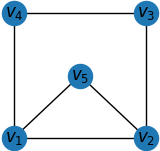
\includegraphics[width=0.4\textwidth]{figures/graph_example.png}}
    \fonte{elaborado pelo autor}
\end{figure}

No exemplo da \autoref{fig:graph_example}, pode se representar o mesmo grafo com $\V = \{v_1, v_2, v_3, v_4, v_5\}$ e $\E = \{\{v_1, v_2\}, \{v_2, v_3\}, \{v_3, v_4\}, \{v_4, v_1\}, \{v_1, v_5\}, \{v_2, v_5\}\}$.
Dentro desse grafo, o subgrafo formato pelos vértices $v_1$, $v_2$ e $v_5$ é também um grafo completo.
A esse conjunto de vértices que forma um subgrafo completo dá-se o nome de clique \cite{fortunato2010community}.
Essa descrição de clique é utilizada como uma definição inicial do conceito de comunidade, partindo de uma perspectiva local \cite{fortunato2010community}.
Dentro desse conceito de comunidade, nomeia-se as arestas cujos dois vértices estão contidos em uma comunidade como sendo interna á comunidade.

É facilmente observável, no entanto, que essa é uma definição muito limitante de comunidade, é raro que comunidades de pessoas apresentem tanta homogeneidade a ponto de todos os membros conhecerem todos os outros membros.
De fato, \citeonline{fortunato2010community} indica que a definição precisa do que é uma comunidade varia de acordo também com o contexto de estudo, mas que algumas características são universais.
Uma comunidade, dentro de qualquer definição, deve ser um sub grafo conexo, por exemplo \cite{fortunato2010community}. 

Algumas das definições alternativas de o que é uma comunidade podem ser expressas.
\citeonline{largeron2015generating} define comunidade como uma classe de estrutura topológica comum a redes complexas, essas comunidades são categorizadas por terem uma densidade de vértices elevada.
O trabalho de \citeonline{shen2009detect} implica que comunidades sejam estruturas que contenham múltiplos cliques dentro de si, e que essas comunidades se dispões em uma estrutura recursiva.
\citeonline{akoglu2009rtg} descreve comunidades como estruturas modulares, onde nodos de um vértice formam grupos distintos entre si por que os membros do grupo tem maior chance de estarem conectados entre si do que estarem conectar com membros de outros grupos.
\citeonline{girvan2002community} define ``Cluster'' e comunidade como duas propriedades distintas, o primeiro sendo a probabilidade de dois nodos ambos adjacentes a um terceiro serem também ajacentes entre si, e a segunda como sendo condutos de vértices densamente conectados entre si, e esparsamente conectados para além de si.

Todas essas definições apresentam características específicas relevantes para a aplicação em que foram utilizadas.
As definições são agrupadas em três classes distintas por \citeonline{fortunato2010community}:

\begin{itemize}
    \item Definição local
    \item Definição global
    \item Definição por similaridade de vértice
\end{itemize}

Essas definições não são mutuamente exclusivas, mas também não são ortogonais uma a outra.
Segundo \citeonline{fortunato2010community}, a definição local parte das características topológicas internas á comunidade.
Nominalmente, isso significa a existência de um conjunto considerável de arestas internas a comunidade e um conjunto limitado de arestas para além da comunidade.

A definição global de comunidades é aplicada aos casos onde a presença de clusters é uma característica inerente ao grafo que se está estudando \citeonline{fortunato2010community}.
Essa propriedade inerente ao grafo pode ser definida como alguma propriedade dos vértices do objeto em questão e que partindo disso se atribui pertencimento á comunidades, ou ainda por comparação com um exemplo nulo \citeonline{fortunato2010community}.
No caso de comparação com um exemplo nulo, define-se uma comunidade pela característica de uma não ser presente dentro de o que é chamado de ``grafo aleatório'' \cite{fortunato2010community}.
Essa definição de um modelo nulo é crucial para o trabalho de \citeonline{girvan2002community}, o modelo nulo considerado é um onde o grafo original é alterado de forma aos graus de todos os vértices se manterem, mas a probabilidade de dois vértices estarem ligados é constante independente de quais os vértices.

A definição de comunidade por similaridade de vértice se baseia na tendencia de que em muitas aplicações, membros de comunidades são mais similares entre si do que seria esperado de um conjunto do mesmo tamanho escolhido aleatoriamente \cite{fortunato2010community}.
Essa definição se faz visível no trabalhos de \citeonline{akoglu2009rtg} e de \citeonline{largeron2015generating}.
Na observação desses dois trabalhos também é interessante o questionamento de como se define semelhança, \citeonline{akoglu2009rtg} representa os vértices como sequencias de caracteres de tamanhos variáveis em que a probabilidade de dois vértices estarem ligados é maior conforme mais caracteres eles compartilham; e \citeonline{largeron2015generating} representa os vértices como pontos em um espaço $n$-dimensional e define que vértices são mais semelhantes quando a distância euclideana deles é menor.

Também independente de qual definição de comunidade que se esteja utilizando, existem os conceitos de partição e cobertura.
Segundo \citeonline{fortunato2010community}, uma partição é uma divisão dos vértices de um grafo tal que cada vértice pertença a um e exatamente um cluster.
O caso de um vértice ``livre'', não pertencendo a nenhuma comunidade, é trivialmente resolvido incluindo ele á comunidade com a qual ele mais tem jacências.
Mas o caso de vértices que pertençam a mais de uma comunidade, i.e. comunidade que se sobreponham, é mais interessante.
\citeonline{fortunato2010community} define uma cobertura como uma divisão dos vértices em clusters onde cada vértice pertence a um ou mais clusters.
\citeonline{fortunato2010community} também descreve o conceito de comunidades hierárquicas, como sendo comunidades cuja estrutura interna também se organiza em clusters de escala menor do que o original.

\citeonline{fortunato2010community} oferece também o conceito de ``função de qualidade'', sendo uma função que mapeia uma partição para um espaço de comparação, usualmente em números reais, onde partições que mapeiem para valores maiores são consideradas melhores.
Segundo \citeonline{fortunato2010community} função de qualidade mais comumente utilizada é a modularidade $Q$ de \citeonline{girvan2002community}.

\begin{quadro}[htb]
\caption{\label{qua:mod_q}Função de modularidade $Q$}

    \begin{equasion}
    \boxed{%
        Q = \frac{1}{2m}\sum_{ij}\Bigg(A_{ij}-\frac{K_iK_j}{2m}\Bigg)\delta(C_i, C_j)
        }
    \end{equasion}

    \fonte{\citeonline{girvan2002community}}
\end{quadro}

Essa função no entanto não se aplica adequadamente ao caso de comunidades sobrepostas ou comunidades hierárquicas, para tanto, é necessário utilizar a função de modularidade estendida, conforme desenvolvido por \citeonline{shen2009detect}.

\begin{quadro}[htb]
\caption{\label{qua:mod_eq}Função de modularidade estendida $EQ$}

    \begin{equasion}
    \boxed{%
        EQ = \frac{1}{2m}\sum_{i}\sum_{v \in C_i, w \in C_i}\frac{1}{O_vO_w}\Bigg[A_{vw} - \frac{K_vK_w}{2m} \Bigg]
        }
    \end{equasion}

    \fonte{\citeonline{shen2009detect}}
\end{quadro}

Tanto no caso da formula descrita no \autoref{qua:mod_q} quanto na do \autoref{qua:mod_eq} a função definida é uma somatórias em que alguns termos se repetem.
Primeiramente, é preciso descrever que a função $\delta(C_iC_j)$ retorna um se $C_i$ for igual a  $C_j$, e zero noutro caso \cite{fortunato2010community}.
Considerando isso, no caso de uma partição (sem comunidades hierárquicas, e sem comunidades sobrepostas), as duas somatórias iteram sobre os mesmos valores, a primeira com os vértices $i$ e $j$ e a segunda com os vértices $v$ e  $w$.

Essa iteração olha para todos os pares de vértices que compartilham alguma comunidade, e soma o valor de $A_{ij}$, sendo $A$ a tabela de adjacência do grafo em questão.
Então é subtraído um valor $\sfrac{K_iK_j}{2m}$, onde  $K_i$ é o grau do vértice $i$ e  $m$ é a quantidade de arestas no grafo ($2m$ portanto é a soma dos graus de todos os vértices).
Esse valor é o a probabilidade de uma aresta entre os vértices  $i$ e  $j$ no modelo nulo de \citeonline{girvan2002community}, considerando que os graus se mantém mas que a probabilidade da presença de uma aresta é uniforme.

A formula $EQ$ de \citeonline{shen2009detect} no entanto contém também o termo escalar $\sfrac{1}{O_vO_w}$, nesse caso o valor $O_i$ é a quantidade de comunidades a qual pertence o vértice $i$.
Isso permite a aplicação da modularidade estendida para os casos de grafos com comunidades sobrepostas.
Vértices que estejam em duas comunidades contribuirão para a modularidade a partir das duas, mas tendo a magnitude da sua contribuição escalada à metade.

\section{Outras propriedades de redes complexas}

Para além da presença de estruturas topológicas que podem ser denominas comunidades, redes complexas tem algumas propriedades topológicas bastante comuns e relevantes.
São algumas delas:

\subsection{Mundo pequeno, Anexação preferencial e Liberdade de escala}

\citeonline{largeron2015generating} descreve a propriedade de mundo pequeno como a característica de um sistema de ter um diâmetro loga ritmicamente proporcional a quantidade de vértices em um grafo.
Isso é, a distancia entre os dois vértices que estão a mais arestas de distância, denominada diâmetro, cresce logaritmicamente conforme observamos exemplos maiores de grafos do sistema.
Essa propriedade implica que em sistemas bastante grandes, é preciso uma quantidade relativamente pequena de saltos de nodo a nodo para se atingir qualquer membro do grafo.

\citeonline{largeron2015generating} define a anexação preferencial como uma propriedade de um sistema em que vértices tendem a se ligar com outros vértices que sejam parecidos e que tenham grau elevado.
Essa propriedade encontra-se presente também no trabalho \citeonline{slota2019scalable}.
Em ambos os casos, a implicação é que dado um sistema onde se vai adicionar um vértice, a maior parte das arestas desse novo vértice devem ligá-lo a outro com grau igual ou maior do que o próprio.

Para atingir essa distribuição característica o modelo de \citeonline{slota2019scalable} faz com que os vértices se dividam em diferentes escalas, de forma que os vértices de uma escala se liguem apenas entre si e com os membros das escalas imediatamente vizinhas.
De grafos com essa distribuição onde o grau relativo de dois vértices adjacentes tende a não apresentar saltos demasiadamente grandes, se diz que são livres de escala \cite{largeron2015generating}.

Essas e uma série de outras proporcionalidades são comumente encontradas em redes complexas.
Outros exemplos de proporcionalidades conhecidas na literatura envolvem os pesos das arestas de um vértice, a proporção de vértices e arestas do grafo e a já citada distribuição dos graus, todas são leis de potência \cite{akoglu2009rtg}.

\subsection{Cluster e comunidades}

\citeonline{girvan2002community} diferencia explicitamente entre a definição de clusters e de comunidades.
No trabalho seminal os autores apontam um cluster como sendo um triângulo, um em outras palavras um subgrafo completo com três vértices.
Essa definição aparentemente arbitrária é relevante no entendimento do coeficiente de clusterização:

\begin{quadro}[htb]
\caption{\label{qua:coecl}Coeficiente de clusterização $C$}

    \begin{equasion}
    \boxed{%
        C = \frac{3 \times (\text{número de triângulos do grafo})}{(\text{número de triplas conexas do grafo})}
        }
    \end{equasion}

    \fonte{\citeonline{girvan2002community}}
\end{quadro}

A conceitualização de um cluster é relevante dentro do estudo de redes complexas na medida em que a implicação é de dois vértices serem ligados por compartilharem uma relação com um terceiro.
O coeficiente $C$ sendo igual a 1 implica que o grafo é um grafo completo \cite{girvan2002community}.
Mais que isso, esse coeficiente, dado um vértice, é a probabilidade de quaisquer dois vértices adjacentes a ele serem adjacentes entre si.

\subsection{Homofilia e Homogeneidade de comunidades}

Conforme foi discutida quanto a definição de comunidades por semelhança de vértices, é de se esperar que vértices adjacentes compartilhem características.
A essa preferência se dá o nome de homofilia \cite{slota2019scalable}.
Essa definição de semelhança é deliberadamente vaga, pois dentro de sistemas distintos é trivial imaginar funções de compatibilidade distintas.
Independentemente disso, observa-se que em grafos obtidos observando sistemas do mundo real, não raro as arestas tornam ajacentes vértices que otimizam alguma função de proximidade, \cite{largeron2015generating}.

Homofilia como propriedade é intimamente ligada a uma outra característica que se observa de grafos do mundo real, em diferentes aplicações as comunidades tendem a ser mais homogêneas do que o grafo ao qual pertencem \cite{largeron2015generating}.
Pode-se afirmar que um grafo onde isso ocorra tem a propriedade de ``comunidades homogêneas''.

\begin{figure}[htpb]
    \centering
    \caption{Exemplo de grafo com comunidades hierárquicas}\label{fig:graph_hier_com}
    \fbox{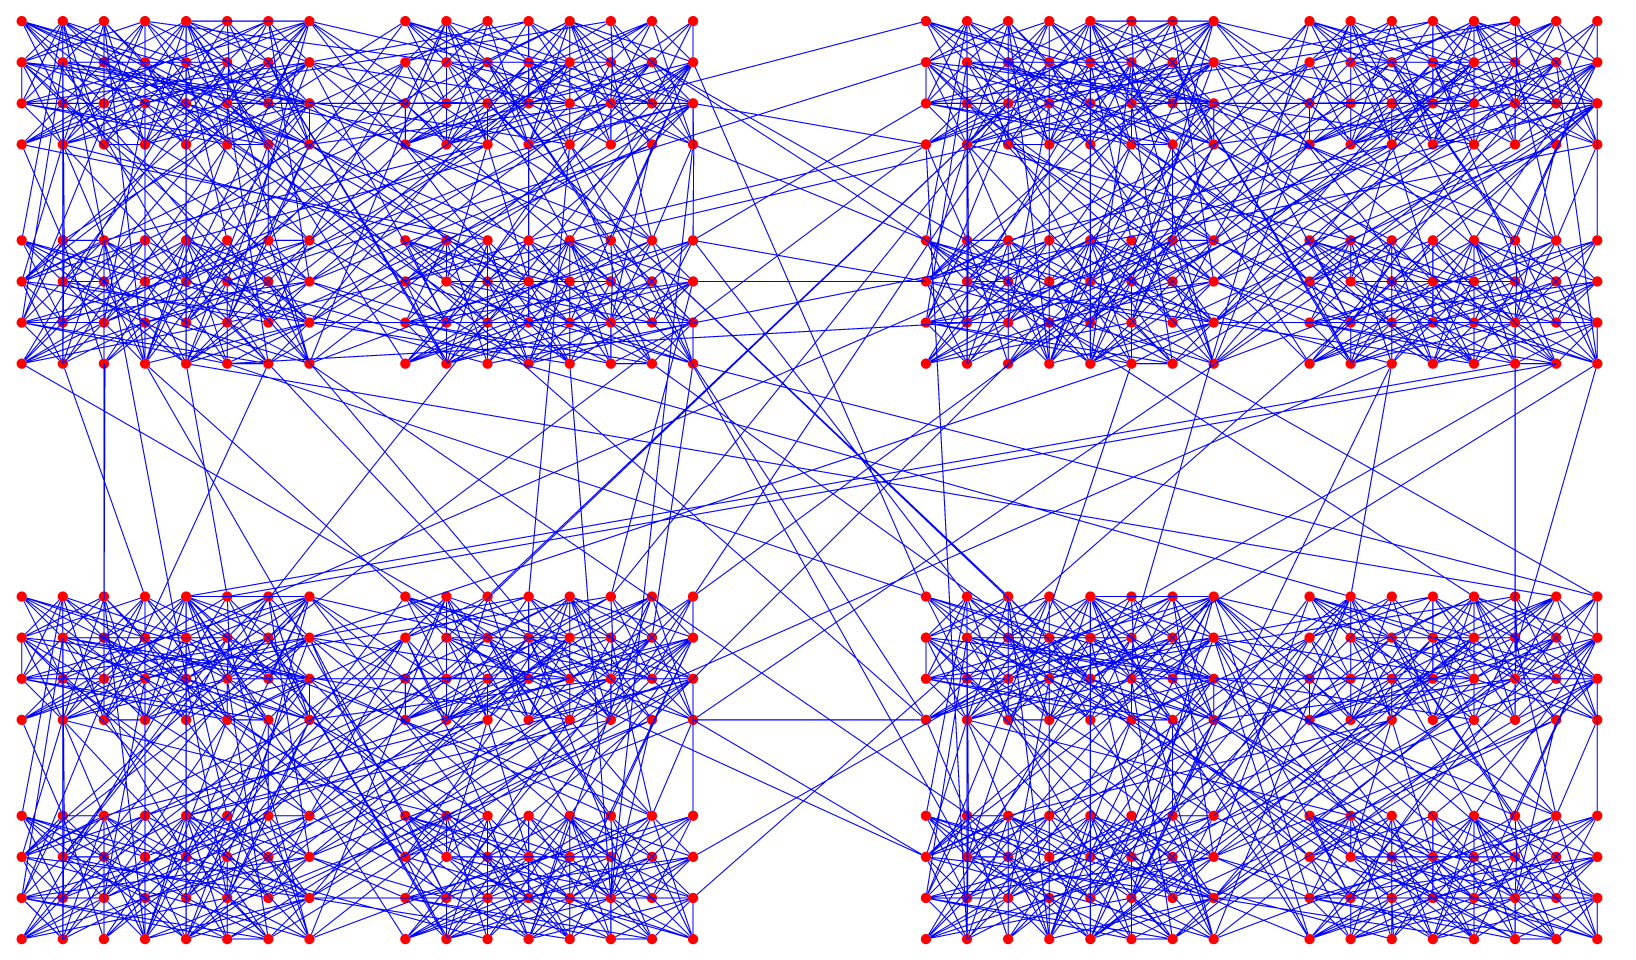
\includegraphics[width=0.8\textwidth]{figures/fortunato2010community_exemplo_comunidades_h.png}}
    \fonte{\citeonline{fortunato2010community}}
\end{figure}

O exemplo da \autoref{fig:graph_hier_com} demonstra como a homofilia as vezes pode ter a presença visualmente verificada.
Se considerarmos que a posição dos vértices na imagem corresponde a duas características ortogonais, a distância entre os vértices pode ser interpretada como uma função de similaridade de dois vértices.
Nesse caso é intuitivamente entendido que vértices mais parecidos de conectam mais do que vértices mais dissemelhantes.

\subsection{Agrupamentos hierárquicos e sobreposições}

No exemplo de grafo da \autoref{fig:graph_hier_com} é possível demonstrar um entendimento intuitivo de como comunidades se organizam.
A estrutura topológica de grupos densamente conectados fica visualmente identificável, onde cada quadrante contém uma comunidade coesa.
Também visualmente acessível, cada comunidade desse exemplo tem uma estrutura interna auto semelhante.

Essa construção de estruturas topológicas recursivas é denominada por \citeonline{girvan2002community} como ``meta grupo'', onde as propriedade topológicas relativas a agrupamentos podem ser encontradas se repetindo em em escalas menores dentro das componentes de escalas maiores.
Comunidades podem funcionalmente ser compostas por comunidades menores.
Esse mesmo conceito recebe uma outra nomenclatura nos trabalhos de \citeonline{largeron2015generating, shen2009detect} e \citeonline{fortunato2010community}, onde são descritas como comunidades hierárquicas.

\begin{figure}[htpb]
    \centering
    \caption{Demonstração dos resultados de diferentes algoritmos de detecção em um grafo com comunidades hierárquicas e com sobreposição}\label{fig:graph_hier_over}
    \fbox{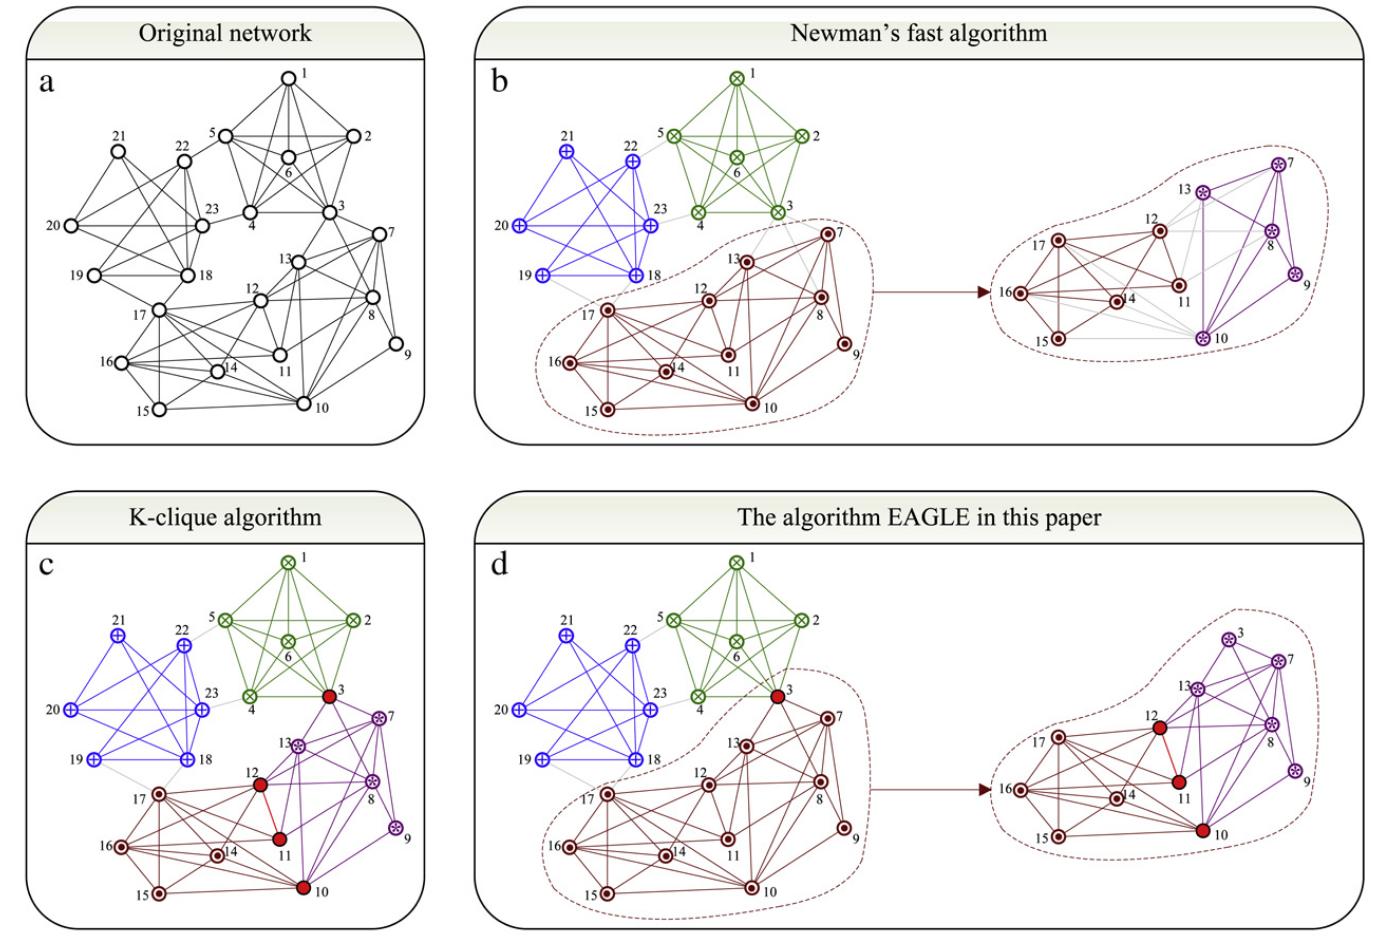
\includegraphics[width=0.8\textwidth]{figures/shen2009detect_graph_com_over.png}}
    \fonte{\citeonline{shen2009detect}}
\end{figure}

Essas estruturas seguem uma característica recursiva, como demonstrado pelo processo de detecção proposto por \citeonline{shen2009detect}, podendo ser concebidos exemplos de sistemas com qualquer sorte de diferentes níveis.
E a elas também se aplica a compreensão de partição ou cobertura, na \autoref{fig:graph_hier_com} as comunidades de primeiro e de segundo nível caracteristicamente não compartilham vértices.
No caso do que demonstra \citeonline{shen2009detect} não só é possível que um vértice pertença a duas comunidades, é possível que ele pertença a duas comunidades de níveis distintos.
Na \autoref{fig:graph_hier_over}, os resultados de \citeonline{shen2009detect} são demonstrados no quadro a respeito do algoritmo EAGLE, o vértice denotado como 3 é compartilhado entre duas comunidades de primeira ordem, mas em uma delas o vértice 3 encontra-se como membro de uma comunidade de segunda ordem.

Ressaltando que a exata definição de comunidade é altamente dependente do contexto \cite{fortunato2010community}, parece ser consenso na literatura que quando se consideram comunidades hierárquicas, todos os membros de uma comunidade de primeiro nível, devem fazer parte de uma das comunidades que compõe a primeira, como observado nos trabalhos de \citeonline{fortunato2010community} e \citeonline{shen2009detect}.
I.e.: nenhum vértice pertence exclusivamente a uma comunidade sem pertencer a alguma das sub comunidades.
Alternativamente claro, o exemplo da \autoref{fig:graph_hier_over} mostra que a implementação de \citeonline{girvan2002community} (quadrante superior direito) é capaz de produzir partições recursivas (note-se a distinção entre uma cobertura e uma partição).

Essa distinção entre cobertura e grafo implica também na definição de comunidades sobrepostas.
Em sistemas do mundo real que produzem redes complexas, é bastante natural que comunidades compartilhem vértices, pois não raro alguma parte de um sistema é componente em dois grupos estruturalmente significantes \cite{shen2009detect}.
Diz-se de duas comunidades que compartilham vértices que elas são comunidades sobrepostas sobrepostas.

O método de detecção de comunidades por K-cliques oferece alguma inspiração no entendimento das propriedades de comunidades sobrepostas.
\citeonline{fortunato2010community} descreve que a forma como esse método trabalha é pivotando subgrafos completos do grafo.
Isso é, dado que um K-clique é um subgrafo completo de $k$ vértices, de dois k-cliques compartilham  $k-1$ vértices, eles devem de fazer parte da mesma comunidade.
Armado desse conhecimento, é possível desenhar que uma cobertura ideal deveria priorizar comunidades com grandes subgrafos completos internamente, mas de que os vértices da intersecção de duas comunidades deveriam de participar de k-cliques distintos, preferencialmente não estando anexos.
A ideia por de trás disso é que se a intersecção de duas comunidades deveria ser parte da periferia das respectivas comunidades \cite{fortunato2010community}.
Se a intersecção fosse tão densamente conexa quando o centro das duas comunidades, esses vértices não seriam mais valore intersectados entre duas comunidades distintas, e as comunidades seriam uma apenas.

\end{document}
